% Technical Documentation: Gravity Storage Electromechanical Simulation
% Compile: pdflatex TECHNICAL_DOCUMENTATION.tex
%           pdflatex TECHNICAL_DOCUMENTATION.tex  (second pass for TOC/refs)
% Requires: pdflatex, standard TeX Live / MiKTeX (tikZ, amsmath, hyperref)

\documentclass[11pt,a4paper]{article}

\usepackage[utf8]{inputenc}
\usepackage[T1]{fontenc}
\usepackage{lmodern}
\usepackage[margin=2.4cm]{geometry}
\usepackage{microtype}
\usepackage{xcolor}
\usepackage{graphicx}
\usepackage{booktabs}
\usepackage{longtable}
\usepackage{array}
\usepackage{amsmath,amssymb}
\usepackage{enumitem}
\usepackage{titlesec}
\usepackage{fancyhdr}
\usepackage{hyperref}
\usepackage{xurl}
\usepackage{adjustbox}
\usepackage{tikz}
\usetikzlibrary{arrows.meta,positioning,shapes.geometric,fit,backgrounds,calc,shadows}

% --- Light theme (print-friendly) ---
\pagecolor{white}
\color{black}
\hypersetup{
  colorlinks=true,
  linkcolor={blue!60!black},
  citecolor={blue!50!black},
  urlcolor={blue!70!black},
  pdfauthor={},
  pdftitle={Technical Documentation: Simulation and Analysis Software}
}
% Allow line breaks in \path/\url at slashes and underscores (file index)
\makeatletter
\g@addto@macro\UrlBreaks{\do\/\do\_\do\-}%
\makeatother

\setlist{itemsep=0.35em,parsep=0pt,topsep=0.4em}
\titleformat{\section}{\normalfont\Large\bfseries}{\thesection}{0.6em}{}
\titleformat{\subsection}{\normalfont\large\bfseries}{\thesubsection}{0.5em}{}

\pagestyle{fancy}
\fancyhf{}
\fancyhead[L]{\small\leftmark}
\fancyhead[R]{\small Technical Documentation}
\fancyfoot[C]{\thepage}
\renewcommand{\headrulewidth}{0.4pt}
\renewcommand{\footrulewidth}{0pt}

\newcommand{\fname}[1]{\texttt{\detokenize{#1}}}

\title{\vspace{-1.2em}\textbf{Technical Documentation}\\[0.35em]
\large Electromechanical Simulation and Multi-Architecture\\Gravitational Energy Storage Analysis Software}
\author{}
\date{\today}

\begin{document}
\maketitle
\thispagestyle{empty}

\begin{abstract}
This document specifies the mathematical models, software architecture, file responsibilities, and data products of the MATLAB-based simulation package. Two complementary layers are described: (1) an ordinary-differential-equation (ODE) electromechanical core for a lumped hoist--drivetrain--motor--electrical load plant, and (2) lumped cycle models for four gravitational storage architectures, integrated in the time domain for comparative energy metrics. All quantities are expressed in SI units unless noted. The objective is complete traceability from physical assumptions to source files and outputs.
\end{abstract}

\vspace{0.8em}
\noindent\textbf{Keywords:} lumped-parameter model, round-trip efficiency, MATLAB, ODE45, gravitational energy storage, regenerative hoist.

\tableofcontents
\newpage

%==============================================================================
\section{Scope and modeling philosophy}
%==============================================================================

The software serves two purposes. First, it integrates a \emph{single-degree-of-freedom} rotational model coupled to a DC-equivalent motor and electrical load, yielding time histories consistent with Newton--Euler dynamics and Kirchhoff--type electrical constraints. Second, it evaluates \emph{architecture-level} energy flows for four conceptually distinct systems by prescribing smooth velocity profiles over operational phases and applying scalar efficiencies and auxiliary power terms, then integrating electrical power.

Lumped-parameter modeling replaces spatially distributed phenomena (fluid fields, magnetic finite elements, multi-segment rope elasticity) with effective masses, phase durations, efficiencies, and bounded auxiliary powers. This is standard when the engineering question is comparative energy accounting under identical gravitational potential budgets rather than subsystem field resolution.

%==============================================================================
\section{Repository structure and execution}
%==============================================================================

The project root contains \fname{setup_path.m}, which adds the repository and subfolders to the MATLAB path. Primary directories:
\begin{itemize}
  \item \fname{models/} --- component functions called by the ODE.
  \item \fname{solvers/} --- \fname{system_ode.m}.
  \item \fname{analysis/} --- \fname{energy_analysis.m}, \fname{validation_checks.m}, \fname{plot_results.m}.
  \item \fname{scripts/} --- runnable drivers, architecture plot scripts, statistical comparison, tiered analysis.
  \item \fname{output/} --- generated tables, figures, and text summaries (when scripts write there).
  \item \fname{docs/} --- supplementary Markdown references (optional reading alongside this PDF).
\end{itemize}

The ODE simulation is invoked by calling \fname{main\_simulation(params)} with \fname{params = system\_parameters()} or a modified structure. Architecture scripts are standalone functions (e.g.\ \fname{plot\_dual\_weight\_results}).

%==============================================================================
\section{System architecture and data flow}
%==============================================================================

Figure~\ref{fig:dfd} shows the layered data flow between parameter files, numerical integrator, component models, and post-processing. Physical power flows along the mechanical chain; algebraic variables couple the electrical port.

\begin{figure}[htbp]
\centering
\begin{adjustbox}{max width=\linewidth,max height=0.38\textheight,center}
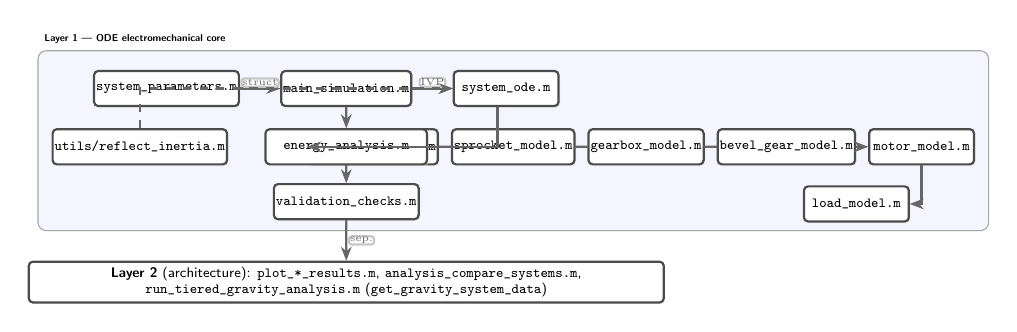
\begin{tikzpicture}[
  scale=0.72, transform shape,
  font=\scriptsize\sffamily,
  box/.style={rectangle, draw=black!70, thick, rounded corners=1.5pt, minimum width=1.85cm, minimum height=0.62cm, align=center, fill=white, inner sep=1pt, drop shadow={shadow xshift=0.6pt, shadow yshift=-0.6pt, fill=black!10}},
  flow/.style={-{Stealth[length=1.8mm]}, thick, black!60},
  lbl/.style={midway, inner sep=0.5pt, fill=white, draw=black!22, rounded corners=1pt, font=\tiny}
]
\node[box] (params) {\fname{system_parameters.m}};
\node[box, right=0.72cm of params] (main) {\fname{main_simulation.m}};
\node[box, right=0.72cm of main] (ode) {\fname{system_ode.m}};
\node[box, below=0.38cm of ode, xshift=-2.35cm] (mass) {\fname{mass_drum_model.m}};
\node[box, right=0.22cm of mass] (spr) {\fname{sprocket_model.m}};
\node[box, right=0.22cm of spr] (gb) {\fname{gearbox_model.m}};
\node[box, right=0.22cm of gb] (bv) {\fname{bevel_gear_model.m}};
\node[box, right=0.22cm of bv] (mot) {\fname{motor_model.m}};
\node[box, below=0.36cm of mot, xshift=-1.15cm] (ld) {\fname{load_model.m}};
\node[box, below=0.38cm of main, minimum width=2.85cm] (ea) {\fname{energy_analysis.m}};
\node[box, below=0.32cm of ea] (val) {\fname{validation_checks.m}};
\node[box, left=0.65cm of ea, minimum width=2.35cm] (refl) {\fname{utils/reflect_inertia.m}};

\draw[flow] (params) -- node[lbl, above=0.5pt] {\tiny struct} (main);
\draw[flow] (main) -- node[lbl, above=0.5pt] {\tiny IVP} (ode);
\draw[flow] (ode.south) ++(-0.15,0) |- (mass.west);
\draw[flow] (mass) -- (spr) -- (gb) -- (bv) -- (mot);
\draw[flow] (mot.south) |- (ld.east);
\draw[flow, dashed] (refl.north) |- (ode.west);

\draw[flow] (main.south) -- (ea.north);
\draw[flow] (ea) -- (val);

\begin{scope}[on background layer]
\node[draw=black!35, rounded corners=3pt, inner sep=5pt, yshift=2pt,
  fit=(params)(main)(ode)(mass)(spr)(gb)(bv)(mot)(ld)(refl), fill=blue!4] {};
\node[anchor=south west, font=\tiny\bfseries\sffamily] at (current bounding box.north west) {Layer 1 --- ODE electromechanical core};
\end{scope}

% Layer 2 (closer to Layer 1 to save vertical space)
\node[box, below=0.72cm of val, minimum width=11.2cm, minimum height=0.72cm, align=center, inner sep=2pt] (arch)
  {\textbf{Layer 2} (architecture): \fname{plot_*_results.m}, \fname{analysis_compare_systems.m},\\\fname{run_tiered_gravity_analysis.m} (\fname{get_gravity_system_data})};
\draw[flow] (val.south) -- node[lbl, right=1pt, font=\tiny] {sep.} (arch.north);

\end{tikzpicture}
\end{adjustbox}
\caption{Layered software and physical signal flow. Layer~1 couples gravitational torque, mechanical train losses, motor electrical equations, and load. Layer~2 uses prescribed kinematics and lumped efficiencies for cross-architecture comparison; it does not call the ODE unless explicitly integrated elsewhere.}
\label{fig:dfd}
\end{figure}

%------------------------------------------------------------------------------
\subsection{Physical signal path (conceptual)}
%------------------------------------------------------------------------------

Figure~\ref{fig:physical} abstracts the plant represented by Layer~1: a point mass moves vertically in one dimension; motion is coupled without slip to a drum; the drum drives a fixed-ratio mechanical train to a rotary electrical machine; the machine terminals connect to an electrical load model.

\begin{figure}[htbp]
\centering
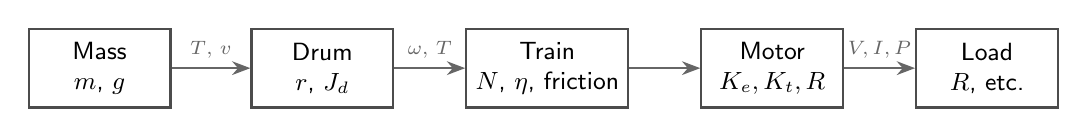
\begin{tikzpicture}[
  font=\small\sffamily,
  blk/.style={rectangle, draw=black!70, thick, minimum height=1.0cm, minimum width=1.8cm, align=center, fill=white},
  arr/.style={-{Stealth}, thick, black!60}
]
\node[blk] (m) {Mass\\$m$, $g$};
\node[blk, right=1.0cm of m] (d) {Drum\\$r$, $J_d$};
\node[blk, right=0.9cm of d] (g) {Train\\$N$, $\eta$, friction};
\node[blk, right=0.9cm of g] (e) {Motor\\$K_e,K_t,R$};
\node[blk, right=0.9cm of e] (l) {Load\\$R$, etc.};
\draw[arr] (m) -- node[above, font=\scriptsize] {$T$, $v$} (d);
\draw[arr] (d) -- node[above, font=\scriptsize] {$\omega$, $T$} (g);
\draw[arr] (g) -- (e);
\draw[arr] (e) -- node[above, font=\scriptsize] {$V,I,P$} (l);
\end{tikzpicture}
\caption{Conceptual electromechanical signal path for Layer~1 (single equivalent vertical DOF coupled to one electrical port).}
\label{fig:physical}
\end{figure}

%==============================================================================
\section{Layer 1: ODE electromechanical core}
%==============================================================================

\subsection{\fname{system\_parameters.m}}

Returns a MATLAB structure grouping: physical constants ($m$, $g$, drum radius and inertia, sprocket ratio and inertia, initial height and velocity); gearbox ratios and inertias; bevel ratio and inertia; motor catalog data ($K_v$, hence $K_e$), winding resistance and inductance, rotor inertia, current limit, optional loss coefficients; per-stage efficiency and Coulomb/viscous friction torques; electrical load type and parameters; ODE solver tolerances and flags (\fname{include\_electrical\_dynamics}, \fname{stop\_at\_bottom}); energy tracking flags; optimization sweep bounds.

Motor voltage constant:
\begin{equation}
K_e = \frac{60}{2\pi\,K_v}\qquad\text{(units: V\,s\,rad$^{-1}$)},\qquad K_t = K_e \quad\text{(SI ideal equality)}.
\end{equation}

Every numeric field is documented inline in the source file with units.

\subsection{\fname{main\_simulation.m}}

\textbf{Initialization.} Converts initial linear speed to drum angular speed $\omega_0 = v_0/r_{\mathrm{drum}}$. Computes total kinematic ratio $N_{\mathrm{tot}}$ from sprocket, gearbox product, and bevel. Sets initial motor speed $\omega_{m,0} = \omega_0/N_{\mathrm{tot}}$. Builds initial state: $[\theta_0,\omega_0,\omega_{m,0}]$ or, if electrical dynamics enabled, appends initial current from \fname{load\_model}.

\textbf{Integration.} Wraps \fname{system\_ode} for the solver; sets relative and absolute tolerances, maximum step, and an event function that fires when height reaches zero downward to terminate the simulation when configured.

\textbf{Post-processing loop.} For each accepted time sample, calls \fname{system\_ode} again with \fname{nargout} requesting component outputs, then \fname{energy\_analysis} to build per-step power and energy metrics.

\textbf{Energy integration.} Trapezoidal accumulation of electrical power and mechanical and electrical loss powers between consecutive samples.

\textbf{Extraction.} Assembles time series for angles, speeds, currents (from state or reconstructed), height, linear speed, mechanical and electrical powers, cumulative energies, and instantaneous efficiency.

\textbf{Conservation check.} Compares initial gravitational energy $mgh_0$ to final electrical energy plus integrated losses plus residual kinetic energy (linear mass term plus rotational contributions from drum, sprocket, gearbox, bevel, motor rotor) to report an energy closure error.

\textbf{Output structure.} Packages all series, parameters copy, timing, final scalar metrics, and passes results to \fname{validation\_checks}.

\textbf{Local helpers.} \fname{system\_ode\_wrapper} adapts ODE signature; \fname{mass\_reached\_bottom} implements the terminal event on height.

\subsection{\fname{solvers/system\_ode.m}}

\textbf{State definition.} $\theta$ drum angle; $\omega$ drum speed; $\omega_m$ motor speed; optional $I$.

\textbf{Electrical branch without inductance dynamics.} Iterative fixed-point solution for $I$ from back-EMF $V_{\mathrm{emf}} = K_e\omega_m$, terminal voltage, and \fname{load\_model}, with current clamped to $I_{\max}$.

\textbf{Bottom stop.} If $h\le 0$ and stopping is enabled, returns zero derivatives and zeroed component outputs for a clean termination state.

\textbf{Mechanical chain.} Sequentially applies \fname{mass\_drum\_model}, \fname{sprocket\_model}, \fname{gearbox\_model}, \fname{bevel\_gear\_model}, \fname{motor\_model}. Re-evaluates current from terminal voltage when not using full electrical state.

\textbf{Inertia aggregation.} Sums reflected inertias to an effective $J$ at the drum using $J/N^2$ relationships consistent with rigid gearing.

\textbf{Kinematic enforcement.} Sets $\omega_m = \omega/N_{\mathrm{tot}}$ and recomputes motor outputs for consistency.

\textbf{Torque balance.} Reflects motor electromagnetic torque to the drum with ratio $N_{\mathrm{tot}}$ and forms net torque $T_{\mathrm{grav}} - T_{m,\mathrm{refl}}$; angular acceleration $\alpha = T_{\mathrm{net}}/J_{\mathrm{tot}}$.

\textbf{State derivatives.} $\dot\theta=\omega$, $\dot\omega=\alpha$, $\dot\omega_m=\alpha/N_{\mathrm{tot}}$; optional $\mathrm{d}I/\mathrm{d}t$ from an $L$--$R$ simplification when enabled. Optional scaling of $\dot\omega_m$ if current exceeds limit (simplified limiter).

\textbf{Component output struct.} Passes heights, velocities, torques, per-stage loss powers, electrical power, motor loss power, currents, voltages, and motor speed for downstream energy accounting.

\subsection{\fname{models/mass\_drum\_model.m}}

Implements:
\begin{align}
h &= \max(0,\; h_0 - r\theta),\\
v &= r\omega,\\
T_{\mathrm{grav}} &= mgr,\\
J_{\mathrm{eff}} &= J_{\mathrm{drum}} + m r^2 .
\end{align}

\subsection{\fname{models/sprocket\_model.m}, \fname{gearbox\_model.m}, \fname{bevel\_gear\_model.m}}

Common pattern per stage: output speed $\omega_{\mathrm{out}}=\omega_{\mathrm{in}}/N$; input power $P_{\mathrm{in}}=T_{\mathrm{in}}\omega_{\mathrm{in}}$; efficiency-scaled power $P'=\eta_{\mathrm{tot}}P_{\mathrm{in}}$ with $\eta_{\mathrm{tot}}=\eta^{n}$ for multi-stage gearbox; friction torque on input shaft combined with viscous term; net power; output torque from $P_{\mathrm{net}}/\omega_{\mathrm{out}}$ when rotating; power loss $P_{\mathrm{in}}-T_{\mathrm{out}}\omega_{\mathrm{out}}$ with non-negativity and sanity clamp; reflected inertia bookkeeping (gearbox sums input inertia plus output and intermediate inertias scaled by cumulative ratio squared).

\subsection{\fname{models/motor\_model.m}}

\begin{align}
V_{\mathrm{emf}} &= K_e \omega_m, &
V_t &= V_{\mathrm{emf}} - IR,\\
T_{\mathrm{em}} &= -K_t I, &
P_{\mathrm{elec}} &= V_t I,\\
P_{\mathrm{Cu}} &= I^2R, &
P_{\mathrm{loss}} &= P_{\mathrm{Cu}} + P_{\mathrm{core}} + P_{\mathrm{bearing}}(\omega_m).
\end{align}

Bearing friction uses Coulomb plus viscous torque multiplied by speed for power; torque is adjusted to include bearing torque directionally.

\subsection{\fname{models/load\_model.m}}

Branches: resistive $I=V_t/R$; battery charging with internal resistance and voltage threshold; constant electrical power demand mapped to $I=P_{\mathrm{in}}/V_t$ with efficiency; custom function handle. Non-negative current clamp and global $I_{\max}$ clamp.

\subsection{\fname{utils/reflect\_inertia.m}}

\begin{equation}
J_{\mathrm{ref}} = J/N^2 .
\end{equation}

\subsection{\fname{analysis/energy\_analysis.m}}

Computes $E_g=mgh$; kinetic contributions at drum and motor; sums mechanical loss powers from sprocket, gearbox, bevel; electrical loss power from motor model; $P_{\mathrm{mech,drum}}=T_{\mathrm{grav}}\omega$; builds nested per-stage power accounting structure; computes instantaneous stage efficiencies and overall $\eta_{\mathrm{system}} = P_{\mathrm{elec}}/P_{\mathrm{mech,drum}}$ with guards against division by zero; returns a complete struct for plotting and tables.

\subsection{\fname{analysis/validation\_checks.m}}

Recomputes end-of-simulation energy balance; checks mass, velocity, current, and voltage ranges for unit sanity; compares peak velocity to free-fall bound $\sqrt{2gh_0}$; validates efficiency bounds; scans for NaN/Inf in state; optionally warns on large numerical acceleration spikes.

\subsection{\fname{analysis/plot\_results.m}}

Optional visualization of \fname{main\_simulation} outputs (see file header comments); not required for numerical core.

%==============================================================================
\section{Layer 2: Architecture cycle models}
%==============================================================================

Each script below defines phase times, smooth normalized velocity profiles $v(t)$, mechanical power where applicable, electrical generation and consumption powers, cumulative energies via trapezoidal integration (\fname{cumtrapz}), and multiple figures (time series, energy summaries, summary tables). Remaining lines configure default graphics colors, axis labels, legends, font names, grid styling, \fname{uitable} summary panels, and restore MATLAB default graphics properties at exit. Those presentation blocks do not alter the underlying power definitions.

\subsection{\fname{scripts/plot\_dual\_weight\_results.m}}

\textbf{Physical story.} Elevator-style cab and counterweight with opposite motion; net imbalance mass $m_{\mathrm{net}}$.

\textbf{Mechanical power.} $P_{\mathrm{mech}} = m_{\mathrm{net}} g (-v_{\mathrm{cab}})$ with descent and ascent windows.

\textbf{Electrical mapping.} Generation interval: $P_{\mathrm{elec}}=\eta_{\mathrm{gen}}\max(P_{\mathrm{mech}},0)$. Ascent motoring: $P_{\mathrm{elec}} = -|P_{\mathrm{mech}}|/\eta_{\mathrm{drive}}$ (negative for consumption convention).

\textbf{Additional series.} Instantaneous regeneration efficiency curve for plotting during descent only; synthetic bounded motor current shape for visualization.

\subsection{\fname{scripts/plot\_variable\_counterweight\_results.m}}

\textbf{Discrete mass schedule.} Integer $n_{\mathrm{modules}}(t)$ controlling attached modules; total mass $m_{\mathrm{tot}}(t)=m_{\mathrm{cabled}}+n_{\mathrm{modules}}m_{\mathrm{module}}$.

\textbf{Descent kinematics.} Smooth $h(t)$ and $v(t)$ from bottom to top of stroke.

\textbf{Main generation.} $P_{\mathrm{mech,main}}=m_{\mathrm{tot}}g(-v)$ on descent; $P_{\mathrm{main,elec}}=\eta_{\mathrm{main,gen}}\max(P_{\mathrm{mech,main}},0)$.

\textbf{Secondary generation event.} Gaussian-shaped power burst timed at module-count transition to represent localized harvesting.

\textbf{Dock buffer discharge.} Positive electrical power waveform during dock phase added to generation total.

\textbf{Ascent motor.} Ideal counterweight mass $m_{\mathrm{ideal}}=m_{\mathrm{cabled}}+m_{\mathrm{module}}$; net load force $\max(0,m_{\mathrm{tot}}g-\lambda m_{\mathrm{ideal}}g)$ with $\lambda<1$ representing imperfect balance; mechanical ascent power is net load times velocity; electrical draw divides by $\eta_{\mathrm{drive}}$ with a minimum power floor.

\textbf{Metrics.} Cumulative consumed (motor) and generated (main + module + supercap branch); round-trip efficiency ratio of totals.

\subsection{\fname{scripts/plot\_buoyancy\_gravity\_results.m}}

\textbf{Lift phase.} Chamber fill state $f(t)\in[0,1]$; motor electrical power reduced as fill increases using a scalar \fname{buoyancy\_fraction} representing effective buoyant support of weight.

\textbf{Water phase.} Weight held at top height; pump electrical load active in a defined temporal window with sinusoidal variation.

\textbf{Drop phase.} Velocity profile yields $P_{\mathrm{gen}}=\eta_{\mathrm{gen}} mg(-v)$.

\textbf{Totals.} Consumption is motor plus pump powers integrated; generation integrates $P_{\mathrm{gen}}$.

\subsection{\fname{scripts/plot\_halbach\_gravity\_results.m}}

\textbf{Lift.} Thrust force scaled with $mg$ and mild variation; mechanical power $F\,v$; electrical lift power divides by $\eta_{\mathrm{lift}}$; constant hoist-hold electrical power during lift and hold to represent rope tension maintenance.

\textbf{Drop.} Same gravitational electrical generation form as other systems.

\textbf{Visualization proxies.} Sinusoidal ``phase current'' for qualitative multi-phase ripple; not an inverter switching model.

\subsection{\fname{scripts/analysis\_compare\_systems.m}}

Reconstructs the same kinematic and power structures as the architecture plot scripts, then executes $n_{\mathrm{rep}}$ replicates with bounded random perturbations of efficiency-like scalars for uncertainty bands. Computes per-replicate energies and efficiencies; performs one-way ANOVA-style sum-of-squares breakdown for efficiency and net energy; writes textual conclusion paths under \fname{output/} when configured; generates comparative figures.

\textbf{Consistency note.} Variable-counterweight statistics in this file may include additional high-power auxiliary consumption terms during dock/load segments relative to the standalone variable-counterweight plot script; numerical results therefore correspond to the analysis script's explicit definitions.

\subsection{\fname{scripts/run\_tiered\_gravity\_analysis.m} and \fname{get\_gravity\_system\_data}}

The nested function \fname{get\_gravity\_system\_data} reproduces the architecture comparison mathematics with an additional per-system multiplicative scale on consumption energies. Tiered figures and text tables summarize round-trip metrics, loss allocations by fixed fractional split of total loss (for reporting), and cost scaling assumptions.

%==============================================================================
\section{Supporting and presentation scripts}
%==============================================================================

\begin{itemize}
  \item \fname{scripts/plot\_figure7\_figure8\_presentation.m} --- Static poster values for energy and efficiency bar charts; exports PNG under \fname{output/}.
  \item \fname{scripts/plot\_figure4\_cycles\_vs\_height.m} --- Parametric curves for scaling behavior vs height.
  \item \fname{scripts/generate\_backboard\_data\_tables.m} --- CSV generation for display tables.
  \item \fname{scripts/run\_example.m}, \fname{scripts/diagnose\_issues.m}, \fname{scripts/optimize\_gearbox.m} --- Example, diagnostic, and parameter sweep utilities invoking \fname{main\_simulation}.
\end{itemize}

%==============================================================================
\section{Equation summary (cross-reference)}
%==============================================================================

Table~\ref{tab:eq} collects recurring forms.

\begin{table}[htbp]
\centering
\caption{Recurring physical and electrical relations.}
\label{tab:eq}
\begin{tabular}{@{}ll@{}}
\toprule
\textbf{Quantity} & \textbf{Relation} \\
\midrule
Gravitational power (translation) & $P \approx mg(-v)$ with sign per convention \\
Drum height & $h=\max(0,h_0-r\theta)$ \\
Motor back-EMF & $V_{\mathrm{emf}}=K_e\omega_m$ \\
Terminal voltage & $V_t=V_{\mathrm{emf}}-IR$ \\
Electrical power & $P_{\mathrm{elec}}=V_t I$ \\
Trapezoidal energy & $E_{n}=E_{n-1}+\tfrac{1}{2}(P_n+P_{n-1})(t_n-t_{n-1})$ \\
Reflected inertia & $J_{\mathrm{ref}}=J/N^2$ \\
\bottomrule
\end{tabular}
\end{table}

%==============================================================================
\section{File index}
%==============================================================================

{\setlength{\tabcolsep}{4pt}\small
\begin{longtable}{@{}>{\raggedright\arraybackslash}p{0.37\textwidth}>{\raggedright\arraybackslash}p{0.57\textwidth}@{}}
\toprule
\textbf{File} & \textbf{Role} \\
\midrule
\endhead
\path|system_parameters.m| & Central SI parameter struct for ODE core. \\
\path|main_simulation.m| & ODE integration driver, energy integration, results struct, terminal event. \\
\path|solvers/system_ode.m| & Coupled mechanical--electrical right-hand side. \\
\path|models/mass_drum_model.m| & $h$, $v$, $T_{\mathrm{grav}}$, $J_{\mathrm{eff}}$. \\
\path|models/sprocket_model.m| & Sprocket ratio, hybrid losses, reflected inertia. \\
\path|models/gearbox_model.m| & Multi-stage ratio, compounded efficiency, friction, inertia reflection. \\
\path|models/bevel_gear_model.m| & Axis redirection stage with losses. \\
\path|models/motor_model.m| & DC-equivalent motor/generator port. \\
\path|models/load_model.m| & Terminal current laws. \\
\path|utils/reflect_inertia.m| & $J/N^2$ helper. \\
\path|analysis/energy_analysis.m| & Instantaneous energy metrics and stage efficiencies. \\
\path|analysis/validation_checks.m| & Conservation and plausibility tests. \\
\path|scripts/plot_dual_weight_results.m| & Dual-mass cycle model and figures. \\
\path|scripts/plot_variable_counterweight_results.m| & Variable-mass cycle model and figures. \\
\path|scripts/plot_buoyancy_gravity_results.m| & Buoyancy-style multi-phase cycle. \\
\path|scripts/plot_halbach_gravity_results.m| & Linear-motor lift + hoist + drop cycle. \\
\path|scripts/analysis_compare_systems.m| & Replicated statistics and comparative figures. \\
\path|scripts/run_tiered_gravity_analysis.m| & Tiered summaries; contains \fname{get_gravity_system_data}. \\
\path|setup_path.m| & MATLAB path configuration. \\
\bottomrule
\end{longtable}
}

%==============================================================================
\appendix
\section{Operational phase abstraction (example)}
%==============================================================================

Figure~\ref{fig:phases} illustrates how architecture scripts partition time into phases with distinct power terms. The numerical values of durations and coefficients reside in the MATLAB sources and may be replaced by measured cycle data.

\begin{figure}[htbp]
\centering
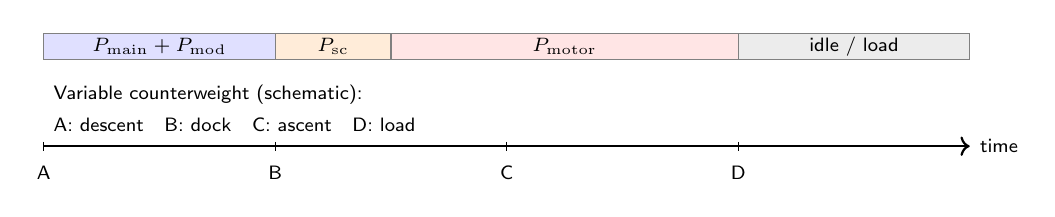
\begin{tikzpicture}[font=\scriptsize\sffamily,x=0.42cm,y=0.55cm]
\draw[->,thick] (0,0) -- (28,0) node[right] {time};
\foreach \x/\lab in {0/A,7/B,14/C,21/D} {\draw (\x,0.1)--(\x,-0.1) node[below=2pt] {\lab};}
\node[anchor=west] at (0,1.2) {Variable counterweight (schematic):};
\node[anchor=west,align=left] at (0,0.5) {A: descent\quad B: dock\quad C: ascent\quad D: load};
\draw[fill=blue!12,draw=black!50] (0,2) rectangle (7,2.6) node[midway] {$P_{\mathrm{main}}+P_{\mathrm{mod}}$};
\draw[fill=orange!15,draw=black!50] (7,2) rectangle (10.5,2.6) node[midway] {$P_{\mathrm{sc}}$};
\draw[fill=red!10,draw=black!50] (10.5,2) rectangle (21,2.6) node[midway] {$P_{\mathrm{motor}}$};
\draw[fill=gray!15,draw=black!50] (21,2) rectangle (28,2.6) node[midway] {idle / load};
\end{tikzpicture}
\caption{Representative power-channel allocation across cycle phases (not to scale).}
\label{fig:phases}
\end{figure}

\section{Extended narrative: \fname{main\_simulation.m} execution order}
%==============================================================================

The function entry optionally supplies \fname{params}; otherwise it calls \fname{system\_parameters}. Initial height and drum radius define the geometric constraint. Initial linear velocity converts to drum angular velocity. The motor initial speed follows the fixed kinematic ratio. The initial state vector is assembled; if full electrical dynamics are disabled, current is not a state variable at $t=0$ beyond what the first \fname{system\_ode} evaluation will infer.

An anonymous function wraps \fname{system\_ode} for the MATLAB ODE solver interface. Solver options include tolerances, maximum step, and an event function that monitors rope-paid height derived from $\theta$. The solver name is selected from \fname{params.simulation.solver}.

After integration, each stored state is reprocessed: \fname{system\_ode} is invoked with the same arguments to recover the component struct consistent with that state, then \fname{energy\_analysis} computes the public energy metrics struct. Cumulative energies integrate instantaneous powers using the trapezoidal rule between consecutive output times.

The results structure duplicates parameters for traceability, stores raw state matrices, exposes convenient aliases for common signals, records conservation metrics, attaches validation output, and includes scalar summaries (final electrical energy, losses, efficiency estimate, drop duration, terminal height).

\section{Symbolic conventions}
%==============================================================================

\begin{itemize}
  \item $\theta,\omega$ --- drum angle and angular velocity.
  \item $\omega_m$ --- motor angular velocity after all fixed ratios.
  \item $N_{\mathrm{tot}}$ --- product of sprocket, gearbox stage, and bevel ratios as implemented.
  \item $P_{\mathrm{elec}}$ --- electrical power at the machine terminals into the defined load convention.
  \item $\eta$ --- per-stage mechanical retention factor applied to shaft power before additional friction subtraction.
\end{itemize}

%==============================================================================
\section*{Document control}
%==============================================================================

\noindent Revision: \today. Generated from repository sources. Export to PDF using \texttt{pdflatex} as described in \fname{latex/README\_COMPILE.txt}.

\end{document}
